\documentclass{article}

\usepackage[usenames]{color}
\usepackage{graphicx}
\usepackage{amsmath}
\usepackage{amsfonts}
\usepackage{amssymb}
\usepackage{mathrsfs}
\usepackage{bm}
\usepackage{verbatim}
\usepackage{cancel}

\begin{document}

\begin{figure}[htbp]

% \centering
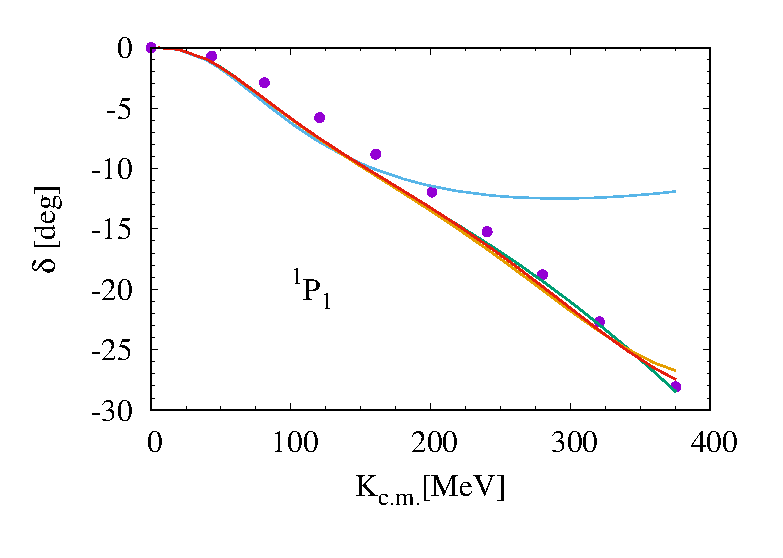
\includegraphics[width=0.5\textwidth]{5_1p1.eps}
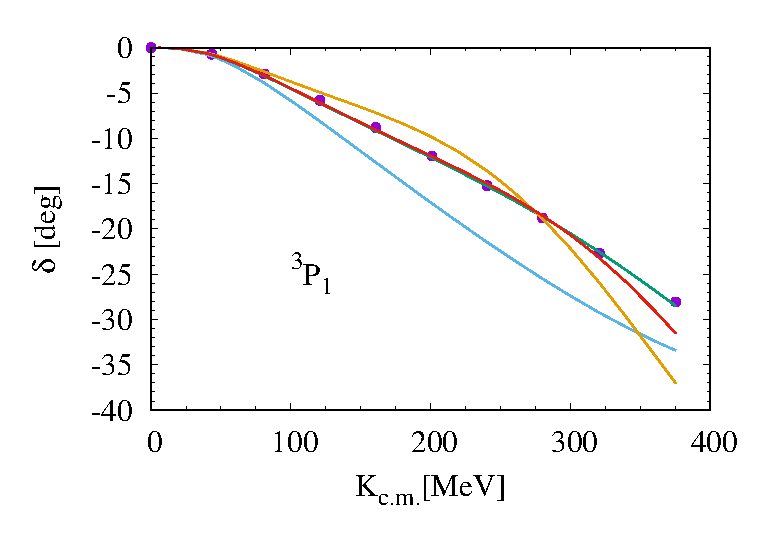
\includegraphics[width=0.5\textwidth]{5_3p1.eps}
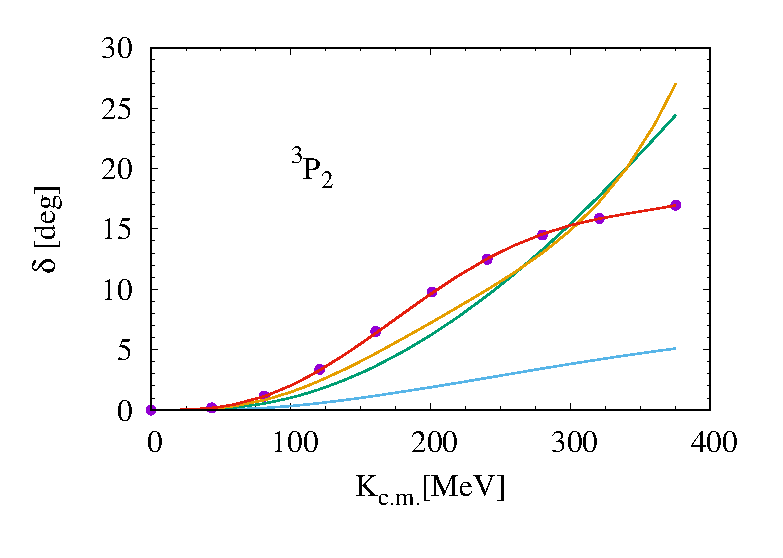
\includegraphics[width=0.5\textwidth]{5_3p2.eps}
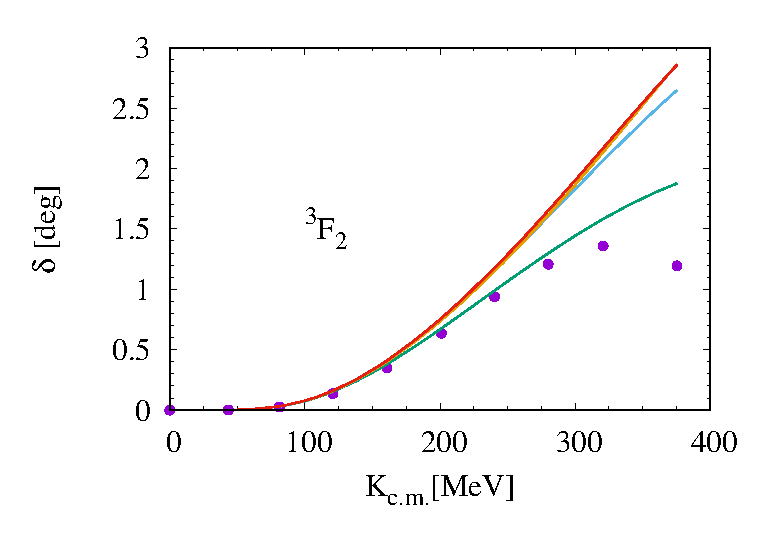
\includegraphics[width=0.5\textwidth]{5_3f2.eps}
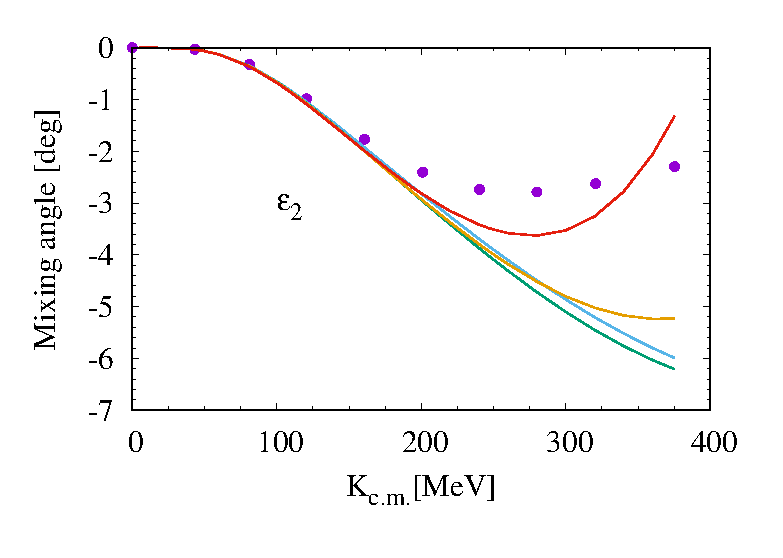
\includegraphics[width=0.5\textwidth]{5_e2.eps}
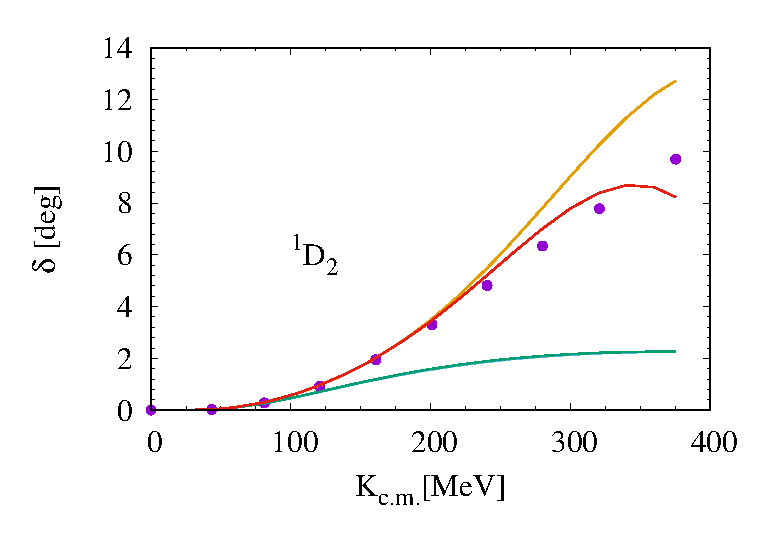
\includegraphics[width=0.5\textwidth]{5_1d2.eps}
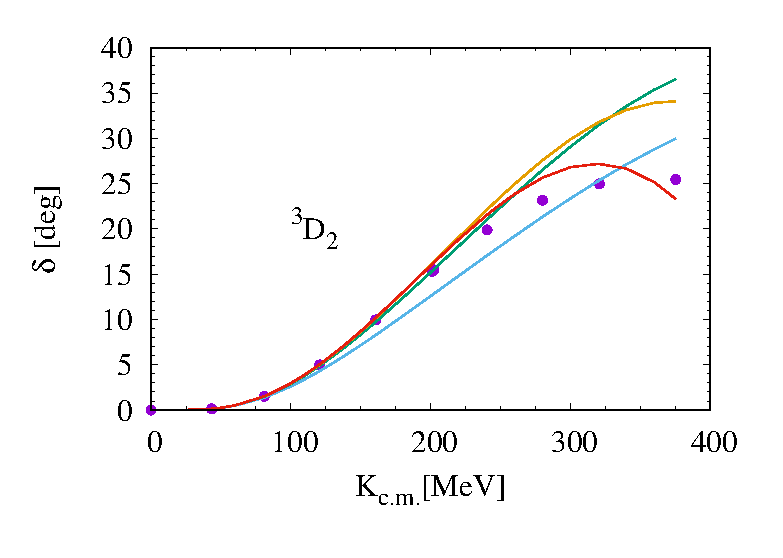
\includegraphics[width=0.5\textwidth]{5_3d2.eps}
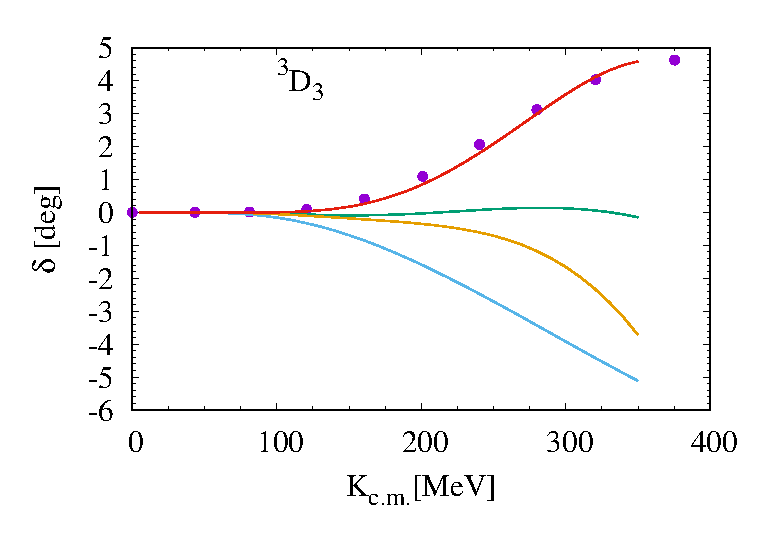
\includegraphics[width=0.5\textwidth]{5_3d3.eps}
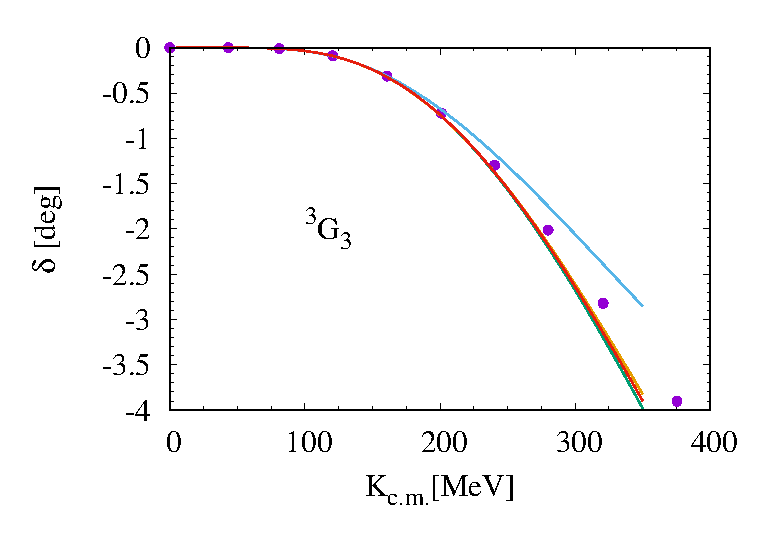
\includegraphics[width=0.5\textwidth]{5_3g3.eps}
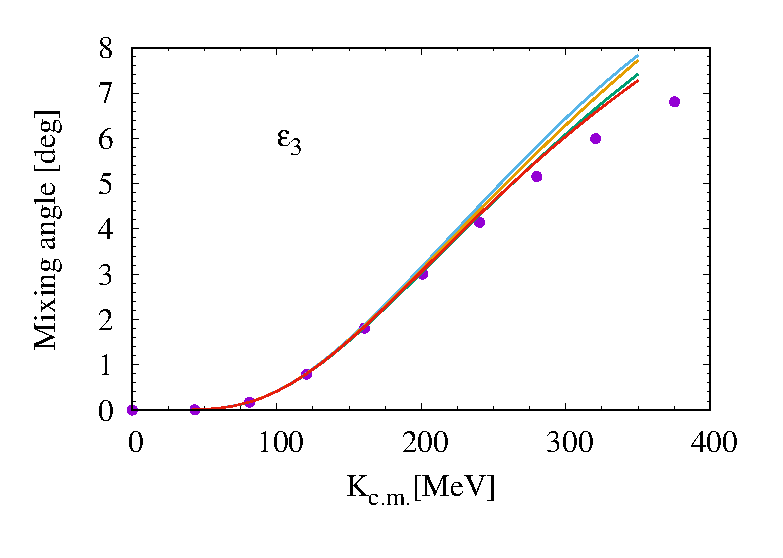
\includegraphics[width=0.5\textwidth]{5_e3.eps}
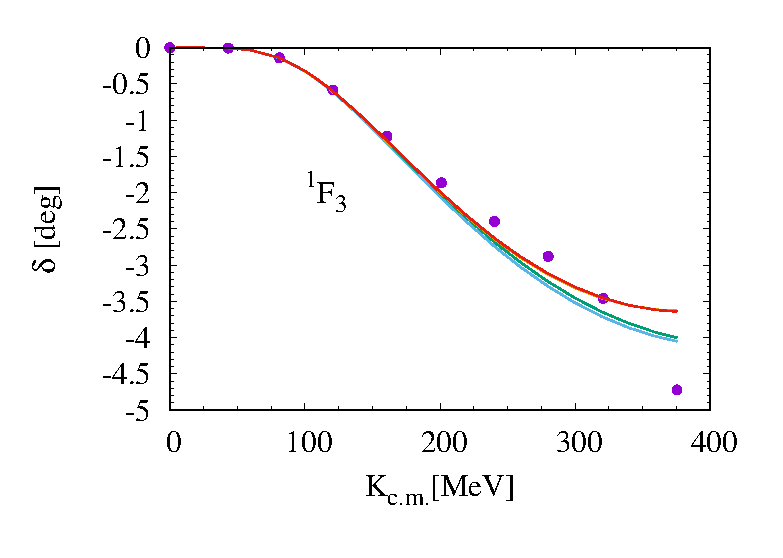
\includegraphics[width=0.5\textwidth]{5_1f3.eps}
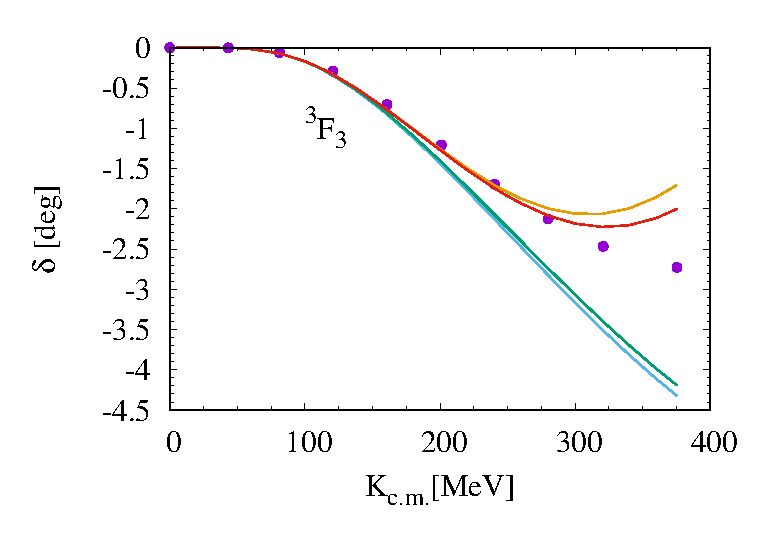
\includegraphics[width=0.5\textwidth]{5_3f3.eps}
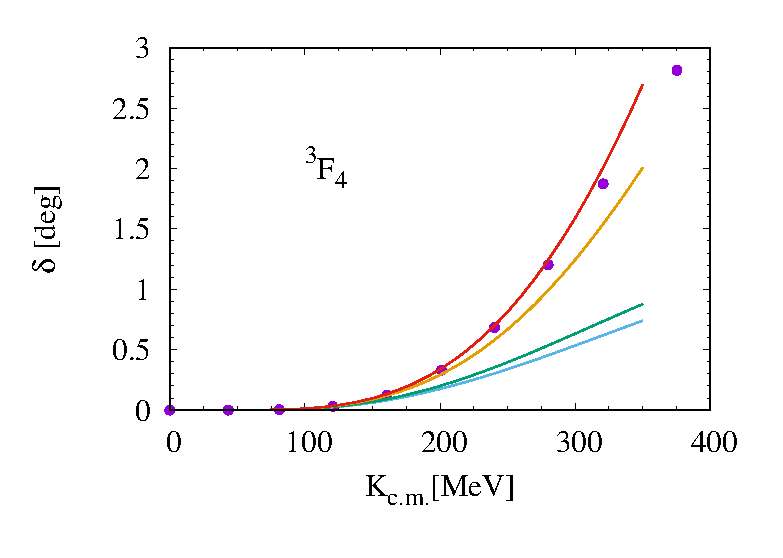
\includegraphics[width=0.5\textwidth]{5_3f4.eps}
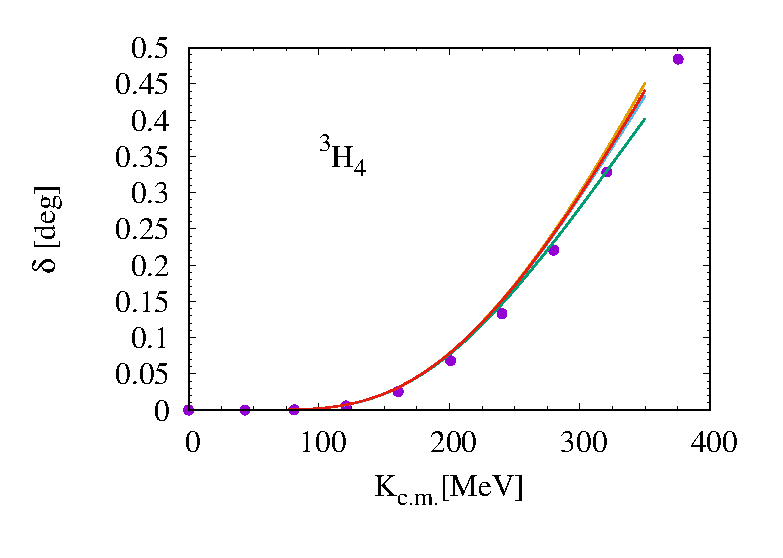
\includegraphics[width=0.5\textwidth]{5_3h4.eps}
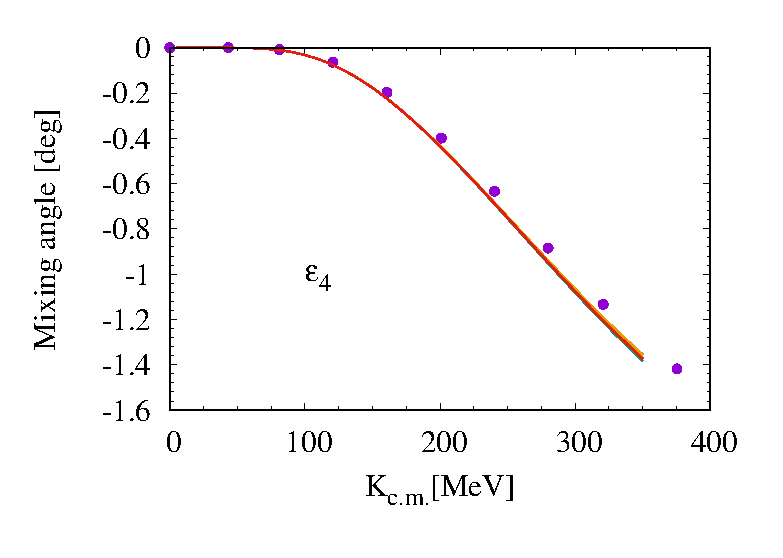
\includegraphics[width=0.5\textwidth]{5_e4.eps}
\caption{The bule, green, orange, and red lines correspond respectively to NLO, N$^2$LO, N$^3$LO, and N$^4$LO. }
% \label{fig:digit}
\end{figure}

\end{document}